%\documentclass{article}
%\usepackage{graphicx,subfigure}
%\begin{document}

\begin{figure}[!h]
  \centering
   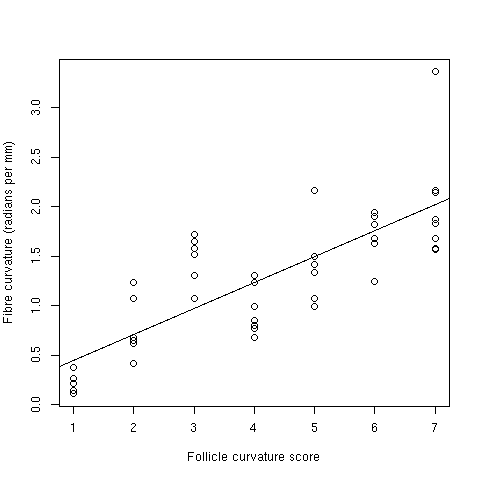
\includegraphics[width=0.9\textwidth]{fig3odr.png}
%  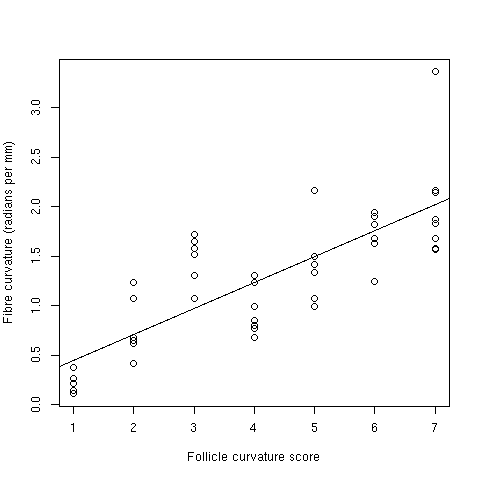
\includegraphics{fig3odr.png}
  \caption{Curvature obtained from the reciprocal transform of radius for number of fibres from  vertical sections of given follicle curvature score. The straight line is the fitted orthogonal regression equation.}
  \label{trandata}
\end{figure}

%\end{document}

